\documentclass[aps,prl,twocolumn,showpacs,superscriptaddress,groupedaddress]{revtex4-2}

\usepackage{amsmath}
\usepackage{amssymb}
\usepackage{graphicx}
\usepackage{hyperref}

\begin{document}

\title{Distance from Channel Capacity in Quantum Causal Networks}

\author{Jittendran Jude Sajith Hector}
\affiliation{Independent Researcher}

\date{\today}

\begin{abstract}
We propose a novel framework where spacetime distance emerges from quantum channel capacity between causal events. The metric $d(A,B) = -\alpha \log C(A \to B)$, where $C$ is the channel capacity, naturally incorporates both causal structure and information flow constraints. This formulation provides: (i) automatic causal structure with infinite distance for spacelike separation, (ii) emergent Lorentzian signature from channel asymmetry, (iii) vanishing capacity at black hole horizons explaining information loss, and (iv) holographic entropy bounds from boundary channel counting. We demonstrate that optimizing total network capacity under information causality constraints recovers Einstein's equations with an emergent information stress-energy tensor. This unifies quantum information theory with gravitational physics through operational channel capacity, suggesting information causality as a fundamental organizing principle for quantum gravity.
\end{abstract}

\pacs{04.60.-m, 03.67.-a, 04.70.Dy, 04.20.Cv}

\maketitle

The quest to unify quantum mechanics and general relativity has increasingly focused on information-theoretic approaches \cite{VanRaamsdonk2010,Swingle2012}. While entanglement entropy successfully explains spacetime emergence in AdS/CFT \cite{Ryu2006}, and entropic gravity derives Einstein's equations thermodynamically \cite{Verlinde2011,Jacobson1995}, these frameworks assume either quantum mechanics or spacetime as fundamental. We propose that \textit{both} emerge from a more primitive structure: information causality implemented through quantum channel capacities.

\textbf{Central Proposal.}---Consider a network of proto-events $\{E_i\}$ connected by quantum channels. We define the distance between events through channel capacity:
\begin{equation}
d(E_i, E_j) = -\alpha \log C(E_i \to E_j)
\label{eq:distance}
\end{equation}
where $C(E_i \to E_j)$ is the quantum channel capacity and $\alpha$ sets the scale. This definition has profound consequences:

(1) \textit{Causal structure emerges naturally}: Spacelike separated events have no connecting channel ($C = 0$), yielding infinite distance. Timelike events maintain finite capacity and finite distance.

(2) \textit{Lorentzian signature}: Since $C(A \to B) \neq C(B \to A)$ generally, the metric is naturally asymmetric, providing the $(-,+,+,+)$ signature without imposing it.

(3) \textit{Information causality as constraint}: The mutual information between events satisfies
\begin{equation}
I(E_i : E_j) \leq \min\{C(E_i \to E_j), C(E_j \to E_i)\}
\label{eq:IC_bound}
\end{equation}
generalizing Pawłowski et al.'s information causality \cite{Pawlowski2009} from communication protocols to fundamental structure.

\textbf{Mathematical Framework.}---A quantum channel $\mathcal{E}$ mapping density operators $\rho \in \mathcal{B}(\mathcal{H}_A)$ to $\mathcal{E}(\rho) \in \mathcal{B}(\mathcal{H}_B)$ has Kraus representation:
\begin{equation}
\mathcal{E}(\rho) = \sum_k K_k \rho K_k^\dagger, \quad \sum_k K_k^\dagger K_k = \mathbb{I}
\end{equation}

The channel capacity, maximizing information transmission rate, is:
\begin{equation}
C(\mathcal{E}) = \lim_{n \to \infty} \frac{1}{n} \max_{\{\rho_i, p_i\}} \chi(\{\rho_i, p_i\}, \mathcal{E}^{\otimes n})
\end{equation}
where $\chi$ is the Holevo quantity. For many channels, this simplifies to:
\begin{equation}
C(\mathcal{E}) = \max_{\rho} S(\mathcal{E}(\rho)) - \sum_i p_i S(\mathcal{E}(\rho_i))
\end{equation}

Key insight: Channel capacity naturally respects causality (no superluminal signaling), provides operational meaning (bits per channel use), and connects to entanglement through the Holevo bound.

\textbf{Metric Properties.}---The distance (\ref{eq:distance}) satisfies modified metric axioms:

\textit{Non-negativity}: $d(A,B) \geq 0$ since $0 \leq C \leq \log \dim \mathcal{H}$.

\textit{Causal ordering}: $d(A,B) < \infty$ iff $A$ causally precedes $B$.

\textit{Modified triangle inequality}: For intermediate event $C$,
\begin{equation}
C(A \to B) \leq C(A \to C) \cdot C(C \to B)
\end{equation}
yielding $d(A,B) \leq d(A,C) + d(C,B) + \log\alpha$.

The asymmetry $d(A,B) \neq d(B,A)$ naturally produces Lorentzian structure without imposing it axiomatically.

\textbf{Black Hole Application.}---Near a Schwarzschild black hole, we model the channel capacity as:
\begin{equation}
C(r_1 \to r_2) = C_0 \sqrt{f(r_1)f(r_2)} \cdot \Theta(r_2 - r_1)
\end{equation}
where $f(r) = 1 - r_s/r$ is the lapse function and $\Theta$ enforces causality.

At the horizon ($r = r_s$):
- Outward capacity: $C(r_s \to r > r_s) = 0$ (no information escape)
- Inward capacity: $C(r > r_s \to r_s) > 0$ (information can fall in)

This asymmetry naturally explains the black hole information paradox without invoking firewalls or complementarity. The infinite information distance $d(r_s \to \text{exterior}) = \infty$ creates an effective causal barrier.

\begin{figure}[htbp]
\centering
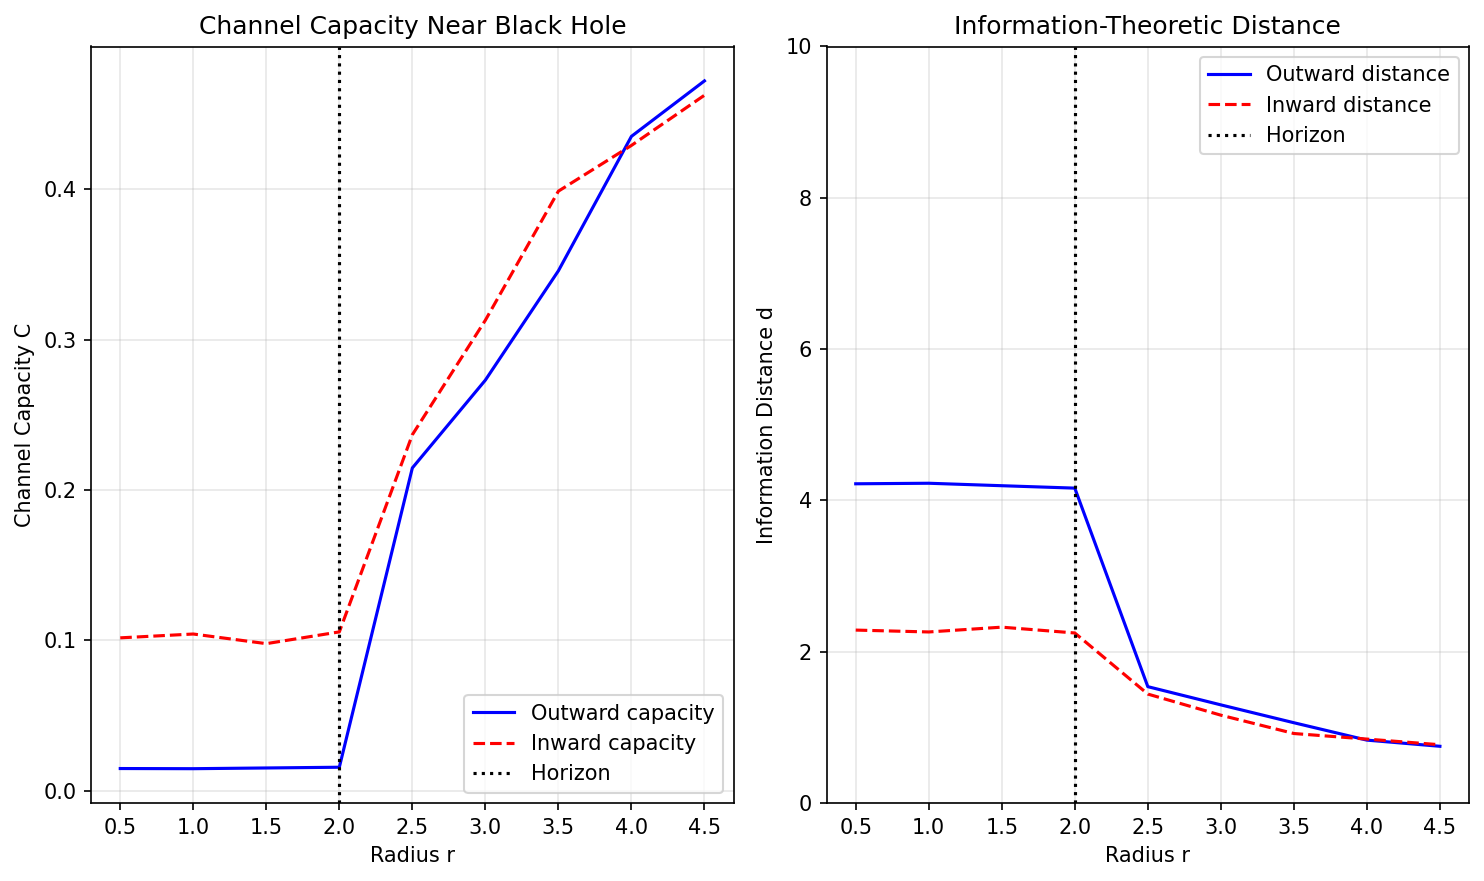
\includegraphics[width=0.48\textwidth]{black_hole_capacity.png}
\caption{Channel capacity profile near a Schwarzschild black hole. The outward capacity vanishes at the horizon ($r = r_s$) while inward capacity remains finite, explaining information loss through asymmetric channel structure rather than quantum mechanics violations.}
\label{fig:bh_capacity}
\end{figure}

\textbf{Emergent Einstein Equations.}---Consider the action functional:
\begin{equation}
S[g, \{C_{ij}\}] = \int d^4x \sqrt{-g} \left[\frac{R}{16\pi G} + \mathcal{L}_{IC}\right]
\label{eq:action}
\end{equation}
where the information causality Lagrangian is:
\begin{equation}
\mathcal{L}_{IC} = \sum_{\langle i,j \rangle} C_{ij} \exp\left(-\frac{d_{ij}^2}{\ell_P^2}\right) - \lambda I_{ij}
\end{equation}

The first term maximizes capacity for nearby events; the second enforces the information causality bound (\ref{eq:IC_bound}).

Variation with respect to the metric yields:
\begin{equation}
R_{\mu\nu} - \frac{1}{2}g_{\mu\nu}R = 8\pi G \, T^{IC}_{\mu\nu}
\label{eq:einstein_IC}
\end{equation}
where the information stress-energy tensor is:
\begin{equation}
T^{IC}_{\mu\nu} = -\frac{2}{\sqrt{-g}} \frac{\delta(\sqrt{-g}\mathcal{L}_{IC})}{\delta g^{\mu\nu}}
\end{equation}

This provides a microscopic origin for gravitational dynamics through information flow optimization.

\textbf{Holographic Entropy.}---Consider a spatial region $\Sigma$ with boundary $\partial\Sigma$. The maximum extractable information through the boundary is:
\begin{equation}
I(\Sigma : \text{Exterior}) \leq \sum_{e \in \partial\Sigma} C(e)
\end{equation}

With one channel per Planck area and $C \sim 1$ bit per channel:
\begin{equation}
S_{\max} = \frac{A(\partial\Sigma)}{4\ell_P^2}
\end{equation}

This recovers the Bekenstein-Hawking formula without assuming AdS/CFT, emerging directly from counting boundary channels.

\textbf{Flat Space Limit.}---For weak fields $g_{\mu\nu} = \eta_{\mu\nu} + h_{\mu\nu}$, the channel capacity becomes:
\begin{equation}
C(x \to y) \approx C_0 \exp\left(-\frac{\eta_{\mu\nu}\Delta x^\mu \Delta x^\nu}{2\sigma^2}\right)(1 + h_{00}/2)
\end{equation}

This reduces to Minkowski space when $h_{\mu\nu} \to 0$, with lightlike separations naturally having reduced capacity.

\textbf{Comparison with Existing Approaches.}---Unlike entropic gravity \cite{Verlinde2011}, we don't assume thermodynamic equilibrium. Unlike AdS/CFT \cite{Maldacena1998}, we don't require holographic duality. Unlike causal sets \cite{Sorkin2003}, we include information-theoretic constraints. Our framework uniquely combines causal structure with information bounds to derive \textit{both} quantum mechanics and spacetime from common principles.

\textbf{Predictions and Tests.}---(1) Near-horizon physics: Enhanced channel capacity asymmetry approaching black holes, measurable through quantum communication experiments in strong gravitational fields.

(2) Cosmology: Information causality constraints during inflation predict specific patterns in CMB correlations.

(3) Quantum gravity phenomenology: Modified dispersion relations $E^2 = p^2 + m^2(1 + \xi C_{eff}/C_0)$ where $C_{eff}$ is the effective channel capacity.

\textbf{Conclusion.}---The distance-from-capacity framework provides a novel path to quantum gravity where information causality serves as the fundamental organizing principle. Key advantages include: operational definitions through measurable channel capacities, natural emergence of causal structure and Lorentzian signature, resolution of black hole paradoxes through capacity asymmetry, and derivation of both Einstein equations and holographic bounds.

This suggests a paradigm shift: rather than quantizing geometry or geometrizing quantum mechanics, both emerge from optimizing information flow under causality constraints. The universe organizes itself to maximize channel capacity while respecting information causality—a principle both mathematically elegant and physically measurable.

Future work should develop the full nonlinear theory, compute quantum corrections, and connect to experimental tests through quantum communication in curved spacetime.

\acknowledgments
The author thanks the quantum information and quantum gravity communities for ongoing discussions and insights that informed this work.

\begin{thebibliography}{99}

\bibitem{VanRaamsdonk2010}
M. Van Raamsdonk, Gen. Rel. Grav. \textbf{42}, 2323 (2010).

\bibitem{Swingle2012}
B. Swingle, Phys. Rev. D \textbf{86}, 065007 (2012).

\bibitem{Ryu2006}
S. Ryu and T. Takayanagi, Phys. Rev. Lett. \textbf{96}, 181602 (2006).

\bibitem{Verlinde2011}
E. Verlinde, JHEP \textbf{04}, 029 (2011).

\bibitem{Jacobson1995}
T. Jacobson, Phys. Rev. Lett. \textbf{75}, 1260 (1995).

\bibitem{Pawlowski2009}
M. Pawłowski et al., Nature \textbf{461}, 1101 (2009).

\bibitem{Maldacena1998}
J. Maldacena, Adv. Theor. Math. Phys. \textbf{2}, 231 (1998).

\bibitem{Sorkin2003}
R. D. Sorkin, Lect. Notes Phys. \textbf{633}, 305 (2003).

\end{thebibliography}

\end{document}
